\begin{figure*}
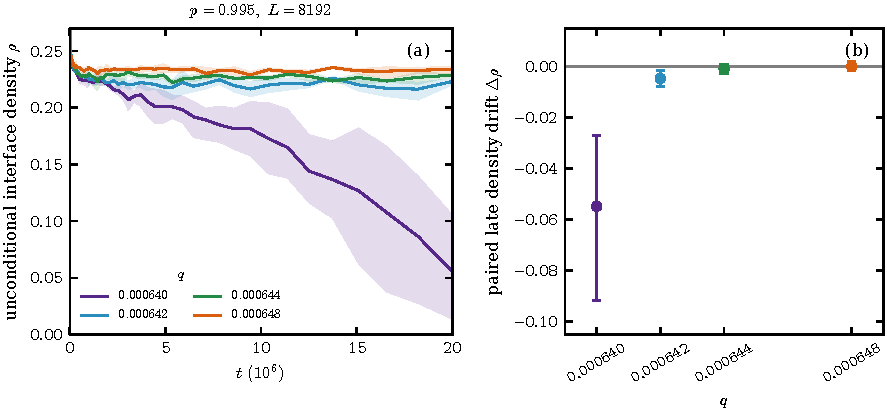
\includegraphics[width=\textwidth]{figs/fig_gpu_near20m}
\caption{Largest-system time dependence near the voter point, $p=0.995$,
$\alpha=1/2$, $L=8192$. All four predeclared independent runs at each actual
$q=0.000640$, 0.000642, 0.000644, and 0.000648 are followed to
$T=2\times10^7$. (a) Unconditional interface density; the trajectory absorbed
at $q=0.000640$ contributes zero for the rest of the horizon.
(b) Paired late drift, the time-weighted mean density over
$1.5\times10^7$--$2\times10^7$ minus that over
$10^7$--$1.5\times10^7$, computed within each run before averaging.
Bands and bars are pointwise 95\% empirical run-bootstrap percentile intervals,
enumerating all 256 ordered resamples of the four runs; their confidence
coverage remains approximate. The midpoint cohort at $q=0.000642$ was declared
independently after the original grid, and is not pooled with other cohorts.
A zero-containing drift interval does not establish stationarity.}
\label{fig:gpu_near20m}
\end{figure*}
